%% Progress slides for the supervisor check of 2026-11-30 (task p10-progress-slides, implementation-plan row 26).
%% Build, from this folder: latexmk -pdf progress-2026-11-30.tex   (build files go to a scratch folder with -outdir=)
%% Every result number is a macro of \resultsdir/results-macros.tex (written by `npm run report -w @breadit/eval`), never typed.
%% The numbers typed here are names and frozen settings of Chapter 3 (K = 10, m = 5, 80% split, 10,000 draws, 0.05, the
%% history group 0--4, the formula constants, the product versions), the same ones Chapter 6 types.
%% The three figures are the pgfplots code of chapters/experiments-and-results.tex, on the same CSV files.
%% The speaker notes are in progress-2026-11-30-notes.md.
\documentclass[aspectratio=169,11pt]{beamer}

%% ── Encoding and packages ────────────────────────────────────────────────────
\usepackage[T1]{fontenc}
\usepackage[utf8]{inputenc}
\usepackage[main=english]{babel}
\usepackage{lmodern}
\usepackage{amsmath}
\usepackage{amssymb}
\usepackage{booktabs}
\usepackage{graphicx}
\usepackage{xcolor}
\usepackage{tikz}
\usetikzlibrary{calc,positioning,arrows.meta}
\usepackage{pgfplots}
\pgfplotsset{compat=1.18}

%% ── A plain theme: white page, one dark blue, no logos of other organisations ─
\usetheme{default}
\definecolor{slideblue}{RGB}{28,60,120}
\setbeamercolor{structure}{fg=slideblue}
\setbeamercolor{frametitle}{fg=slideblue}
\setbeamercolor{block title}{fg=white,bg=slideblue}
\setbeamercolor{block body}{fg=black,bg=slideblue!6}
\setbeamerfont{frametitle}{series=\bfseries,size=\large}
\setbeamerfont{title}{series=\bfseries,size=\large}
\setbeamerfont{block title}{size=\small,series=\bfseries}
\setbeamersize{text margin left=0.9cm,text margin right=0.9cm}
\setbeamertemplate{navigation symbols}{}
\setbeamertemplate{itemize item}{\raisebox{0.15ex}{\scriptsize$\bullet$}}
\setbeamertemplate{itemize subitem}{\raisebox{0.1ex}{\scriptsize$-$}}
\setbeamertemplate{enumerate item}{\insertenumlabel.}
\setbeamertemplate{blocks}[rounded][shadow=false]
\setbeamertemplate{frametitle}{%
  \vskip2mm\nointerlineskip
  \usebeamerfont{frametitle}\usebeamercolor[fg]{frametitle}\insertframetitle\par
  \vskip0.8mm{\color{slideblue}\hrule height 0.6pt}}
\setbeamertemplate{footline}{%
  \hbox to\paperwidth{\hspace{0.9cm}{\color{gray}\scriptsize Breadit\ \textperiodcentered\ progress check\ \textperiodcentered\ 2026-11-30}\hfill
  {\color{gray}\scriptsize\insertframenumber\,/\,\inserttotalframenumber}\hspace{0.9cm}}\vskip3mm}
\setlength{\parskip}{3pt}
\renewcommand{\arraystretch}{1.15}

%% ── Results, the same way as main.tex ────────────────────────────────────────
\newcommand{\resultsdir}{../../results/p7-report}
\input{\resultsdir/results-macros.tex}

%% The title registered with the school (the same text as main.tex).
\newcommand{\thesistitle}{Breadit: A real-time hybrid social networking platform with social-graph-aware personalized feed ranking}

%% Screenshot by name: \slideshot{<name>}{<width>}{<height>} shows ../images/<name>.png (or .pdf) if it exists,
%% else a framed placeholder with the file name, like \thesisdiagram of main.tex. The deck builds either way.
\newcommand{\slideshot}[3]{%
  \IfFileExists{../images/#1.png}{\includegraphics[width=#2,height=#3,keepaspectratio]{../images/#1.png}}{%
  \IfFileExists{../images/#1.pdf}{\includegraphics[width=#2,height=#3,keepaspectratio]{../images/#1.pdf}}{%
  \fbox{\parbox[c][#3][c]{\dimexpr#2-2\fboxsep-2\fboxrule\relax}{\centering\small Screenshot to add:\\[2pt]\footnotesize\texttt{#1.png}\\ in \texttt{../images/}}}}}}

%% ── Filters and look of the three figures (copied from chapters/experiments-and-results.tex) ──
\pgfplotsset{
  discard if not/.style 2 args={
    x filter/.code={
      \edef\resfigtempa{\thisrow{#1}}%
      \edef\resfigtempb{#2}%
      \ifx\resfigtempa\resfigtempb\else\def\pgfmathresult{inf}\fi
    }
  },
  discard if/.style 2 args={
    x filter/.code={
      \edef\resfigtempa{\thisrow{#1}}%
      \edef\resfigtempb{#2}%
      \ifx\resfigtempa\resfigtempb\def\pgfmathresult{inf}\fi
    }
  },
  keep rows/.style n args={4}{
    x filter/.code={
      \edef\resfigtempa{\thisrow{#1}}%
      \edef\resfigtempb{#2}%
      \edef\resfigtempc{\thisrow{#3}}%
      \edef\resfigtempd{#4}%
      \ifx\resfigtempa\resfigtempb\else\def\pgfmathresult{inf}\fi
      \ifx\resfigtempc\resfigtempd\def\pgfmathresult{inf}\fi
    }
  },
  gainplot/.style={
    height=4.5cm,
    width=0.36\textwidth,
    tick label style={font=\scriptsize},
    label style={font=\scriptsize},
    title style={font=\footnotesize},
    ylabel={Gain in NDCG@10 ($H - \mathrm{BL2}$)},
    scaled y ticks=false,
    yticklabel style={/pgf/number format/fixed, /pgf/number format/fixed zerofill, /pgf/number format/precision=2},
    extra y ticks={0},
    extra y tick labels={},
    extra y tick style={grid=major, grid style={dashed, black!70}},
    error bars/y dir=both,
    error bars/y explicit,
    error bars/error bar style={thick},
    error bars/error mark options={rotate=90, mark size=2pt},
    every axis plot/.append style={black, only marks, mark size=2pt},
  },
}

\title[Breadit]{\thesistitle}
\subtitle{Progress check}
\author{Cao Ngoc Anh Tuan -- ITCSIU21244}
\institute[IU]{School of Computer Science and Engineering\\The International University, VNU-HCM}
\date{2026-11-30}
\titlegraphic{\IfFileExists{../images/IU.png}{
\includegraphics[height=1.7cm]{../images/IU.png}}{}}

\begin{document}

%% ── 1. Title ─────────────────────────────────────────────────────────────────
\begin{frame}[plain]
  \titlepage
  \vspace{-2mm}
  \centering{\small Supervisor: MSc. Nguyen Trung Nghia}
\end{frame}

%% ── 2. Problem and research questions ────────────────────────────────────────
\begin{frame}
  \frametitle{The problem and the research questions}
  \begin{itemize}
    \item ``For You'' in Breadit shows the posts of you and your followees, newest first. The follow graph does not decide which post comes first.
    \item Explore uses one engagement score for everyone (likes, comments, reposts, age), not the follow graph.
    \item A new user has no history, so there is little to personalize with.
  \end{itemize}
  \vspace{1mm}
  \begin{block}{RQ1}
    Does adding social-graph signals (follow trust and community affinity) to the ranking improve the ``For You'' feed over the current heuristic, especially for users with little history?
  \end{block}
  \begin{block}{RQ2}
    How does the level of social interaction between users change the ranking quality? What is the minimum level where the social signal starts to help?
  \end{block}
\end{frame}

%% ── 3. Hypotheses ────────────────────────────────────────────────────────────
\begin{frame}
  \frametitle{The hypotheses, frozen before the first test run}
  \small
  \begin{block}{H1 (RQ1)}
    For users with 0--4 earlier interactions, the hybrid has higher NDCG@10 than BL2. It passes if the paired 95\% confidence interval of the difference is above 0 after Holm correction. Two co-primary tests, each with this pass rule and each reported on its own: test 1 on synthetic data (the middle cell of world W2, size M: \texttt{syn-W2M-M}), test 2 on real data (Digg 2009: \texttt{digg2009}).
  \end{block}
  \begin{block}{H2 (RQ2)}
    The gain over BL2 grows with social density (number of followees, amount of friend engagement in the pool). It is about zero when the user follows nobody and has no community.
  \end{block}
  \begin{block}{H0 (sanity gate)}
    In the null world W0 (follows are random), H-follow must not beat BL2. A win means a bug or a leak.
  \end{block}
  \footnotesize If a hypothesis fails, the thesis reports it as it is.
\end{frame}

%% ── 4. Architecture ──────────────────────────────────────────────────────────
\begin{frame}
  \frametitle{The system: one ranking code for the app and for the evaluation}
  \centering
  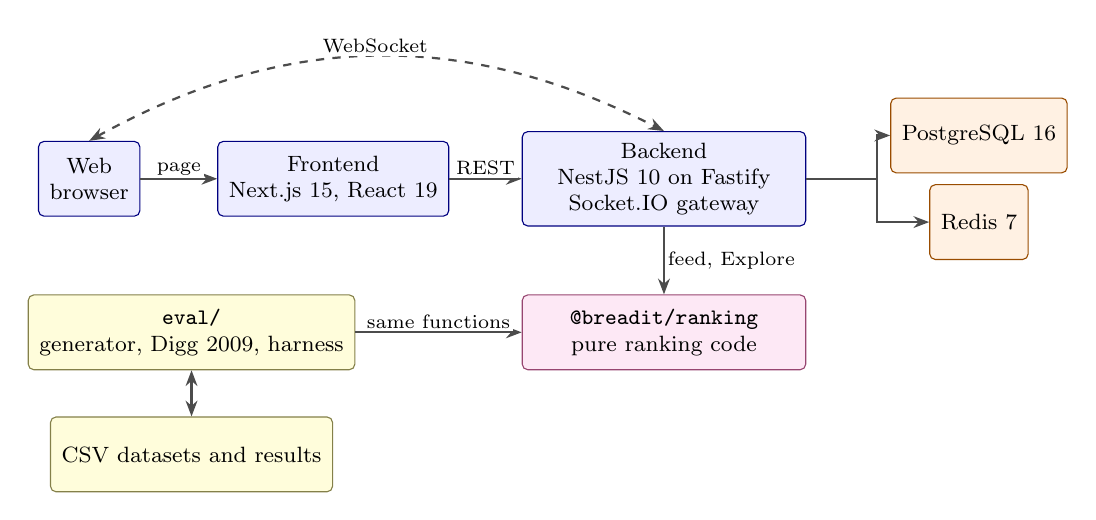
\begin{tikzpicture}[
      box/.style={draw, rounded corners=2pt, align=center, inner sep=4pt, font=\footnotesize, minimum height=0.95cm},
      app/.style={box, fill=blue!7, draw=blue!50!black},
      pkg/.style={box, fill=magenta!9, draw=magenta!55!black},
      evl/.style={box, fill=yellow!14, draw=yellow!45!black},
      sto/.style={box, fill=orange!11, draw=orange!60!black},
      >={Stealth[length=2mm]},
      link/.style={->, thick, draw=black!70},
      lab/.style={font=\scriptsize, fill=white, inner sep=1pt}]
    \node[app] (br) at (0.9,3.7) {Web\\browser};
    \node[app] (fe) at (4.0,3.7) {Frontend\\Next.js 15, React 19};
    \node[app, minimum width=3.6cm] (be) at (8.2,3.7) {Backend\\NestJS 10 on Fastify\\Socket.IO gateway};
    \node[sto] (pg) at (12.2,4.25) {PostgreSQL 16};
    \node[sto] (rd) at (12.2,3.15) {Redis 7};
    \node[pkg, minimum width=3.6cm] (rk) at (8.2,1.75) {\texttt{@breadit/ranking}\\pure ranking code};
    \node[evl, minimum width=3.4cm] (ev) at (2.2,1.75) {\texttt{eval/}\\generator, Digg 2009, harness};
    \node[evl] (cs) at (2.2,0.2) {CSV datasets and results};
    \draw[link] (br) -- node[lab, above] {page} (fe);
    \draw[link] (fe) -- node[lab, above] {REST} (be);
    \draw[link, <->, dashed] (br.north) to[bend left=28] node[lab, above] {WebSocket} (be.north);
    \draw[link] (be.east) -- ($(be.east)+(0.9,0)$) |- (pg.west);
    \draw[link] (be.east) -- ($(be.east)+(0.9,0)$) |- (rd.west);
    \draw[link] (be) -- node[lab, right] {feed, Explore} (rk);
    \draw[link] (ev) -- node[lab, above] {same functions} (rk);
    \draw[link, <->] (ev) -- (cs);
  \end{tikzpicture}
  \par\vspace{1mm}
  \begin{itemize}\setlength\itemsep{0pt}\small
    \item Nothing imports \texttt{eval/}. The harness never uses Postgres, Redis or HTTP.
    \item \texttt{@breadit/ranking} has no Nest, Prisma, Redis, clock or random numbers.
  \end{itemize}
\end{frame}

%% ── 5. Real-time layer and the three feeds ───────────────────────────────────
\begin{frame}
  \frametitle{The real-time layer and the three feeds}
  \begin{columns}[T]
    \begin{column}{0.48\textwidth}
      \textbf{Real-time (Socket.IO)}
      \begin{itemize}\small
        \item One gateway with the Redis adapter. It reads the session cookie in the handshake.
        \item Each user joins a room named after the username.
        \item Services push events: notifications, direct messages (rooms \texttt{conversation:<id>}, typing dots), and \texttt{accountBanned}, which logs a banned user out at once.
      \end{itemize}
    \end{column}
    \begin{column}{0.48\textwidth}
      \textbf{Three \texttt{algo} feeds on ``For You''}
      \begin{itemize}\small
        \item \texttt{chrono} (BL0): followee posts first, newest first.
        \item \texttt{engagement} (BL2): the Explore score on the shared pool.
        \item \texttt{social} (H): the hybrid score.
        \item The cursor is \texttt{t:score:id}, so every page ranks at the same time $t$.
        \item The default is set by \texttt{FEED\_DEFAULT\_ALGO}. Unset, ``For You'' is as it was.
      \end{itemize}
    \end{column}
  \end{columns}
  \vspace{2mm}
  \begin{block}{Parity test}
    The live feed and the evaluation call the same package. The parity test checks that the live order equals the harness order.
  \end{block}
\end{frame}

%% ── 6. The hybrid score ──────────────────────────────────────────────────────
\begin{frame}
  \frametitle{The hybrid score $H$}
  \small
  \[ H(p,u,t) = \mathrm{engagement}(p,t) + \alpha \cdot \mathrm{social}(p,u,t) + \beta \cdot \mathrm{community}(p,u,t) \]
  \vspace{-4mm}
  \begin{align*}
    \mathrm{engagement}(p,t) &= \text{likes} + 2\cdot\text{comments} + 3\cdot\text{reposts} - 0.25\cdot\text{ageHours} \quad(=\text{BL2})\\
    \mathrm{social}(p,u,t) &= \mathbf{1}[u \text{ follows } a(p)]\cdot\mathrm{trust}(u,a(p),t) + \sum_{f\ \text{engaged before}\ t}\mathrm{trust}(u,f,t)\\
    \mathrm{trust}(u,f,t) &= \frac{n_{uf} + m/|F_u|}{N_u + m}\\
    \mathrm{community}(p,u,t) &= \frac{c_{u,c(p)} + m\cdot\mathbf{1}[u \text{ is a member of } c(p)]\,/\,|M_u|}{N_u + m}
  \end{align*}
  \vspace{-4mm}
  \begin{itemize}\footnotesize
    \item $a(p)$: the author of $p$. $n_{uf}$: earlier positives of $u$ on posts by $f$. $N_u$: all earlier positives of $u$. $F_u$: followees. $M_u$: communities. $c_{u,c}$: earlier positives of $u$ in community $c$.
    \item The prior $m = 5$ (frozen): a user with no history gives every followee the same trust, $1/|F_u|$, so the score is defined for new users. Its weight falls as history grows.
    \item $\alpha$ and $\beta$ were tuned on validation items only. On \texttt{syn-W2M-M}: $\alpha / \beta$ = \tuneWTwoMHChosen{}, the values in the live \texttt{social} feed.
  \end{itemize}
\end{frame}

%% ── 7. Data ──────────────────────────────────────────────────────────────────
\begin{frame}
  \frametitle{Data: two sources, because each tests what the other cannot}
  \begin{columns}[T]
    \begin{column}{0.48\textwidth}
      \textbf{Synthetic worlds} (seeded generator)
      \begin{itemize}\small
        \item W0: the null world, follows are random.
        \item W1: similar users follow each other, no influence.
        \item W2L, W2M, W2H: low, middle and high influence. W2M is H1 test 1.
        \item Size M. The generator never ranks a feed, so the data do not depend on any tested method.
        \item The only data with communities.
      \end{itemize}
      Test users of \texttt{syn-W2M-M}: \eOneWTwoMTestUsersAllN{} (left out of the pool: \eOneWTwoMLeftOutAllN{}).
    \end{column}
    \begin{column}{0.48\textwidth}
      \textbf{Digg 2009} (real data)
      \begin{itemize}\small
        \item Dated follows and dated votes on one clock. A vote counts as a like.
        \item A follow counts for a test only if it is dated before the test time.
        \item No communities, so $\beta$ has no effect.
        \item Small and special: one month, only stories that reached the front page. The zips come from an Internet Archive copy.
        \item H1 test 2.
      \end{itemize}
      Test users of \texttt{digg2009}: \eOneDiggTestUsersAllN{} (left out: \eOneDiggLeftOutAllN{}).
    \end{column}
  \end{columns}
\end{frame}

%% ── 8. Protocol ──────────────────────────────────────────────────────────────
\begin{frame}
  \frametitle{Protocol and statistics}
  \begin{columns}[T]
    \begin{column}{0.52\textwidth}
      \textbf{Protocol}
      \begin{itemize}\footnotesize
        \item \textbf{Temporal split.} One cut time $T$ at 80\% of all positives. Tune before $T$, test after $T$, once.
        \item \textbf{One test item per user:} the last positive after $T$ on a post the user had not touched.
        \item \textbf{As-of rule.} Every feature uses only events before the test time. A leakage test checks it.
        \item \textbf{Pool.} The same \texttt{buildPool} as the live feed. The whole pool is ranked, with no sampled negatives.
        \item \textbf{Metrics.} NDCG@10 is the main one (also Recall and Coverage at $K$ = 5, 10, 20). Gain = mean paired difference $H - \text{BL2}$.
        \item \textbf{Baselines} BL0 to BL6. BL2 is the production Explore score. BL4 (Reddit) and BL5 (Hacker News) are strong time-decay formulas. BL2t, BL4, BL5 and BL6 are tuned like $H$.
      \end{itemize}
    \end{column}
    \begin{column}{0.44\textwidth}
      \textbf{Statistics}
      \begin{itemize}\footnotesize
        \item Paired bootstrap 95\% interval and paired randomization test, 10,000 draws each, seeded.
        \item Holm correction inside each family. F1 is $H - \text{BL2}$.
        \item \textbf{H1 passes on a dataset only if} the Holm-adjusted $p$ is below 0.05 \textbf{and} the lower end of the interval is above 0 (NDCG@10, group 0--4).
        \item \textbf{Default feed rule:} ``For You'' becomes \texttt{social} only if H1 passes on both tests and the H0 gate passes.
      \end{itemize}
      \vspace{1mm}
      \textbf{Reproducible}
      \begin{itemize}\footnotesize
        \item One command, \texttt{npm run thesis:repro}, rebuilds every result and compares each file with a hash manifest.
      \end{itemize}
    \end{column}
  \end{columns}
\end{frame}

%% ── 9. H0 gate and E1 ────────────────────────────────────────────────────────
\begin{frame}
  \frametitle{Results: the H0 gate, then all methods (E1)}
  \begin{columns}[T]
    \begin{column}{0.46\textwidth}
      \begin{block}{H0 gate: passes}
        \small H-follow against BL2 on W0: gain \hZeroWZeroNdcgHFollowTenAllGain{}, 95\% interval from \hZeroWZeroNdcgHFollowTenAllCiLow{} to \hZeroWZeroNdcgHFollowTenAllCiHigh{}. The interval contains 0, so follows that are random do not help. The other results can be used.
      \end{block}
      \begin{itemize}\small
        \item \texttt{syn-W2M-M}: $H$ reaches \eOneWTwoMNdcgHTenAllValue{}, BL2 only \eOneWTwoMNdcgBLTwoTenAllValue{}.
        \item \texttt{digg2009}: $H$ and BL2 are equal (\eOneDiggNdcgHTenAllValue{} and \eOneDiggNdcgBLTwoTenAllValue{}). The ``hot'' baselines BL4 and BL5 are far better.
      \end{itemize}
    \end{column}
    \begin{column}{0.50\textwidth}
      \centering
      \small NDCG@10 on the test split, all users\\[1mm]
      \footnotesize
      \begin{tabular}{lrr}
        \toprule
        Method & \texttt{syn-W2M-M} & \texttt{digg2009} \\
        \midrule
        BL0  & \eOneWTwoMNdcgBLZeroTenAllValue{}  & \eOneDiggNdcgBLZeroTenAllValue{} \\
        BL1  & \eOneWTwoMNdcgBLOneTenAllValue{}   & \eOneDiggNdcgBLOneTenAllValue{} \\
        BL2  & \eOneWTwoMNdcgBLTwoTenAllValue{}   & \eOneDiggNdcgBLTwoTenAllValue{} \\
        BL2t & \eOneWTwoMNdcgBLTwoTTenAllValue{}  & \eOneDiggNdcgBLTwoTTenAllValue{} \\
        BL3  & \eOneWTwoMNdcgBLThreeTenAllValue{} & \eOneDiggNdcgBLThreeTenAllValue{} \\
        BL4  & \eOneWTwoMNdcgBLFourTenAllValue{}  & \eOneDiggNdcgBLFourTenAllValue{} \\
        BL5  & \eOneWTwoMNdcgBLFiveTenAllValue{}  & \eOneDiggNdcgBLFiveTenAllValue{} \\
        BL6  & \eOneWTwoMNdcgBLSixTenAllValue{}   & \eOneDiggNdcgBLSixTenAllValue{} \\
        \midrule
        $H$  & \textbf{\eOneWTwoMNdcgHTenAllValue{}} & \textbf{\eOneDiggNdcgHTenAllValue{}} \\
        \bottomrule
      \end{tabular}
    \end{column}
  \end{columns}
\end{frame}

%% ── 10. H1 ───────────────────────────────────────────────────────────────────
\begin{frame}
  \frametitle{H1 fails on both co-primary tests (E2)}
  \centering
  \small
  Gain of $H$ over BL2 in NDCG@10, history group 0--4\\[1.5mm]
  \footnotesize
  \begin{tabular}{lrrrrrl}
    \toprule
    Test & Users & Gain & CI low & CI high & Holm $p$ & H1 \\
    \midrule
    \texttt{syn-W2M-M} & \eTwoWTwoMNdcgTenZeroFourN{} & \eTwoWTwoMNdcgTenZeroFourGain{} & \eTwoWTwoMNdcgTenZeroFourCiLow{} & \eTwoWTwoMNdcgTenZeroFourCiHigh{} & \eTwoWTwoMNdcgTenZeroFourPHolm{} & fails \\
    \texttt{digg2009}  & \eTwoDiggNdcgTenZeroFourN{} & \eTwoDiggNdcgTenZeroFourGainFull{} & \eTwoDiggNdcgTenZeroFourCiLowFull{} & \eTwoDiggNdcgTenZeroFourCiHighFull{} & \eTwoDiggNdcgTenZeroFourPHolm{} & fails \\
    \bottomrule
  \end{tabular}
  \par\vspace{2mm}
  \raggedright\small
  \begin{itemize}
    \item \textbf{\texttt{syn-W2M-M}:} the gain is positive, but the interval contains 0 and the Holm $p$ is above 0.05. There are few users in the group, so the interval is wide.
    \item \textbf{\texttt{digg2009}:} the lower end of the interval is above 0, but only by a very small amount (six decimals shown). The Holm $p$ is above 0.05. H1 needs both conditions.
    \item The only row of family F1 at $K = 10$ where both conditions hold is the opposite of the hope: users of \texttt{syn-W2M-M} with 20 or more earlier interactions gain \eTwoWTwoMNdcgTenTwentyPlusGain{} (interval \eTwoWTwoMNdcgTenTwentyPlusCiLow{} to \eTwoWTwoMNdcgTenTwentyPlusCiHigh{}, Holm $p$ \eTwoWTwoMNdcgTenTwentyPlusPHolm{}).
  \end{itemize}
\end{frame}

%% ── 11. Figure E2 ────────────────────────────────────────────────────────────
\begin{frame}
  \frametitle{E2: the gain by history group}
  \centering
  \begin{tikzpicture}
    \begin{axis}[
      name=left, gainplot,
      title={\texttt{syn-W2M-M}},
      xlabel={History group},
      symbolic x coords={0,1-4,0-4,5-19,20+},
      xtick={0,1-4,0-4,5-19,20+},
      xticklabels={0,1--4,0--4,5--19,20+},
    ]
      \addplot[black] table[col sep=comma, x=bin, y=mean_diff,
        y error plus expr=\thisrow{ci_high}-\thisrow{mean_diff},
        y error minus expr=\thisrow{mean_diff}-\thisrow{ci_low},
        discard if not={dataset}{syn-W2M-M}]{\resultsdir/fig-e2-history.csv};
    \end{axis}
    \begin{axis}[
      at={(left.east)}, anchor=west, xshift=1.9cm, gainplot,
      title={\texttt{digg2009}},
      xlabel={History group},
      symbolic x coords={0,1-4,0-4,5-19,20+},
      xtick={0,1-4,0-4,5-19,20+},
      xticklabels={0,1--4,0--4,5--19,20+},
      scaled y ticks=base 10:4,
      yticklabel style={/pgf/number format/fixed, /pgf/number format/fixed zerofill, /pgf/number format/precision=0},
    ]
      \addplot[black] table[col sep=comma, x=bin, y=mean_diff,
        y error plus expr=\thisrow{ci_high}-\thisrow{mean_diff},
        y error minus expr=\thisrow{mean_diff}-\thisrow{ci_low},
        discard if not={dataset}{digg2009}]{\resultsdir/fig-e2-history.csv};
    \end{axis}
  \end{tikzpicture}
  \par\vspace{1mm}
  \raggedright\footnotesize
  Marks: mean gain with the 95\% interval, $K = 10$. The dashed line is 0. Group 0--4 is the group of H1. \texttt{digg2009} is on its own, much smaller scale.\par
  \small On \texttt{syn-W2M-M} the gain grows with history: \eTwoWTwoMNdcgTenZeroFourGain{} in group 0--4 and \eTwoWTwoMNdcgTenTwentyPlusGain{} in group 20+. On Digg it is near 0 in every group.
\end{frame}

%% ── 12. Figure E3 ────────────────────────────────────────────────────────────
\begin{frame}
  \frametitle{E3: the gain by social density (H2)}
  \centering
  \begin{tikzpicture}
    \begin{axis}[
      name=left, gainplot,
      title={W2 cells (synthetic)},
      xlabel={Followees},
      symbolic x coords={0,1-4,5-19,20+},
      xtick={0,1-4,5-19,20+},
      xticklabels={0,1--4,5--19,20+},
      legend style={font=\scriptsize, at={(0.5,-0.32)}, anchor=north, legend columns=-1},
    ]
      \addplot[black, xshift=-5pt, mark=triangle*, mark options={solid, fill=white}] table[col sep=comma, x=bin, y=mean_diff,
        y error plus expr=\thisrow{ci_high}-\thisrow{mean_diff},
        y error minus expr=\thisrow{mean_diff}-\thisrow{ci_low},
        keep rows={dataset}{syn-W2L-M}{n}{1}]{\resultsdir/fig-e3-density.csv};
      \addlegendentry{W2L}
      \addplot[black, xshift=0pt, mark=*] table[col sep=comma, x=bin, y=mean_diff,
        y error plus expr=\thisrow{ci_high}-\thisrow{mean_diff},
        y error minus expr=\thisrow{mean_diff}-\thisrow{ci_low},
        keep rows={dataset}{syn-W2M-M}{n}{1}]{\resultsdir/fig-e3-density.csv};
      \addlegendentry{W2M}
      \addplot[black, xshift=5pt, mark=square*, mark options={solid, fill=white}] table[col sep=comma, x=bin, y=mean_diff,
        y error plus expr=\thisrow{ci_high}-\thisrow{mean_diff},
        y error minus expr=\thisrow{mean_diff}-\thisrow{ci_low},
        keep rows={dataset}{syn-W2H-M}{n}{1}]{\resultsdir/fig-e3-density.csv};
      \addlegendentry{W2H}
    \end{axis}
    \begin{axis}[
      at={(left.east)}, anchor=west, xshift=1.9cm, gainplot,
      title={\texttt{digg2009}},
      xlabel={Followees},
      symbolic x coords={0,1-4,5-19,20+},
      xtick={0,1-4,5-19,20+},
      xticklabels={0,1--4,5--19,20+},
      scaled y ticks=base 10:4,
      yticklabel style={/pgf/number format/fixed, /pgf/number format/fixed zerofill, /pgf/number format/precision=0},
    ]
      \addplot[black] table[col sep=comma, x=bin, y=mean_diff,
        y error plus expr=\thisrow{ci_high}-\thisrow{mean_diff},
        y error minus expr=\thisrow{mean_diff}-\thisrow{ci_low},
        discard if not={dataset}{digg2009}]{\resultsdir/fig-e3-density.csv};
    \end{axis}
  \end{tikzpicture}
  \par\vspace{1mm}
  \raggedright\footnotesize
  Bin 1--4 holds too few users in the W2 cells and has no mark. The dashed line is 0.\par
  \small The gain is already there at 0 followees (W2L \eThreeWTwoLNdcgTenZeroGain{}, W2M \eThreeWTwoMNdcgTenZeroGain{}, W2H \eThreeWTwoHNdcgTenZeroGain{}) and is lower at 20 or more (\eThreeWTwoLNdcgTenTwentyPlusGain{}, \eThreeWTwoMNdcgTenTwentyPlusGain{}, \eThreeWTwoHNdcgTenTwentyPlusGain{}). \textbf{H2 is not supported.}
\end{frame}

%% ── 13. Figure E5 ────────────────────────────────────────────────────────────
\begin{frame}
  \frametitle{E5: is the result built into the data?}
  \centering
  \begin{tikzpicture}
    \begin{axis}[
      gainplot,
      width=0.88\textwidth,
      height=4.9cm,
      symbolic x coords={syn-W0-M,syn-W1-M,syn-W2L-M,syn-W2M-M,syn-W2H-M,h0-gate,topic-signal,shuffled,own-tuning,syn-W2M-M-shuffled},
      xmin=syn-W0-M, xmax=shuffled,
      enlarge x limits=0.08,
      xtick={syn-W0-M,syn-W1-M,syn-W2L-M,syn-W2M-M,syn-W2H-M,h0-gate,topic-signal,shuffled},
      xticklabels={W0,W1,W2L,W2M,W2H,{W0, H-follow (gate)},{W0, W2M values},{W2M, shuffled}},
      xticklabel style={rotate=25, anchor=east},
      legend style={font=\scriptsize, at={(0.02,0.97)}, anchor=north west},
      legend cell align=left,
    ]
      \addplot[black, mark=*] table[col sep=comma, x=dataset, y=mean_diff,
        y error plus expr=\thisrow{ci_high}-\thisrow{mean_diff},
        y error minus expr=\thisrow{mean_diff}-\thisrow{ci_low},
        discard if not={variant}{own-tuning}]{\resultsdir/fig-e5-worlds.csv};
      \addlegendentry{Each world with its own tuning}
      \addplot[black, mark=square*, mark options={solid, fill=white}] table[col sep=comma, x=variant, y=mean_diff,
        y error plus expr=\thisrow{ci_high}-\thisrow{mean_diff},
        y error minus expr=\thisrow{mean_diff}-\thisrow{ci_low},
        discard if={variant}{own-tuning}]{\resultsdir/fig-e5-worlds.csv};
      \addlegendentry{Control runs}
    \end{axis}
  \end{tikzpicture}
  \par
  \raggedright\small
  \begin{itemize}\setlength\itemsep{0pt}
    \item The gain grows with the influence in the data: W0 \eFiveWZeroNdcgTenAllGain{}, W1 \eFiveWOneNdcgTenAllGain{}, W2L \eFiveWTwoLNdcgTenAllGain{}, W2M \eFiveWTwoMNdcgTenAllGain{}, W2H \eFiveWTwoHNdcgTenAllGain{}.
    \item W0 and W1 have no influence and still gain: the community term acts as a topic signal. Shuffled engagement times keep most of the gain (\eFiveWTwoMShuffledNdcgTenAllGain{} against \eFiveWTwoMNdcgTenAllGain{}).
  \end{itemize}
\end{frame}

%% ── 14. E7 cost ──────────────────────────────────────────────────────────────
\begin{frame}
  \frametitle{E7: the cost of the three feeds}
  \centering
  \small Page 1 of each \texttt{algo}, one machine, page cache off, one virtual user\\[2mm]
  \small
  \resizebox{0.95\textwidth}{!}{\input{\resultsdir/tables/e7.tex}}
  \par\vspace{2mm}
  \raggedright
  \begin{itemize}\small
    \item The intervals overlap: this setup shows no difference in time between the three feeds. The median is \eSevenSocialMedian{}~ms for \texttt{social}.
    \item The three feeds run the same queries (on average \eSevenChronoQueriesMean{}, \eSevenEngagementQueriesMean{} and \eSevenSocialQueriesMean{} Prisma queries per request).
    \item This is a repeatable result, not an identical one (timings change a little between runs). It says nothing about many users at once.
  \end{itemize}
\end{frame}

%% ── 15. What it means (1) ────────────────────────────────────────────────────
\begin{frame}
  \frametitle{What it means (1): the answers to RQ1 and RQ2}
  \begin{itemize}\small
    \item \textbf{RQ1: not on these data.} H1 fails on both tests.
    \begin{itemize}
      \item Few users in group 0--4 (\eTwoWTwoMNdcgTenZeroFourN{} on \texttt{syn-W2M-M}), so a small gain cannot be told from 0.
      \item With no history, every followee gets the same trust. The score says ``someone you follow'', not which one the user likes. The gain grows with history.
      \item On Digg, our reading is that the social term is small next to the vote counts (not tested). What works there is time decay (BL4, BL5), not the follow graph.
    \end{itemize}
    \item \textbf{RQ2: no level where it starts to help.} The gain is already there at 0 followees and does not rise (H2 not supported).
    \item \textbf{What the hybrid really uses (E4).} On \texttt{syn-W2M-M}, H-comm gains \eFourWTwoMNdcgHCommTenAllGain{} of the \eFourWTwoMNdcgHTenAllGain{} of the full score. H-follow gains only \eFourWTwoMNdcgHFollowTenAllGain{}.
    \begin{itemize}
      \item In the generator a community is a topic, so the community term works as a topic-interest signal. It is real personalization, but it is not the social signal that RQ1 asked about.
    \end{itemize}
  \end{itemize}
\end{frame}

%% ── 16. What it means (2) ────────────────────────────────────────────────────
\begin{frame}
  \frametitle{What it means (2): for Breadit, and the limits}
  \begin{columns}[T]
    \begin{column}{0.48\textwidth}
      \textbf{For Breadit}
      \begin{itemize}\small
        \item \textbf{The default feed stays as it is.} H1 failed, so the rule keeps ``For You'' unchanged. \texttt{algo=social} stays as an option. A later study can change the default with one variable, no new code.
        \item \textbf{Cost is not the reason} (E7).
        \item \textbf{The offline numbers are about the live code}: same package, parity test.
        \item A stronger time decay may help Explore, but only on some data. It needs its own test. Future work.
      \end{itemize}
    \end{column}
    \begin{column}{0.48\textwidth}
      \textbf{Limits}
      \begin{itemize}\small
        \item Synthetic data: we wrote the generator, and a community is a topic in it.
        \item Digg is small, special and has no communities.
        \item No real data for the community term (the Hive data refused access).
        \item Small group 0--4. The tuned $\alpha$ and $\beta$ sit at the edge of the grid.
        \item Offline test: one item per user. It does not measure whether users are happier.
      \end{itemize}
    \end{column}
  \end{columns}
\end{frame}

%% ── 17. Demo plan ────────────────────────────────────────────────────────────
\begin{frame}
  \frametitle{The demo plan}
  \small
  Data: \texttt{syn-W2M-M} moved to today, in the Postgres schema \texttt{eval\_demo} and Redis database 3. Start with \texttt{npm run demo:start}. Two browser windows: A is a normal window (a user with long history), B is a private window (a user with little history).
  \begin{enumerate}\small
    \setlength\itemsep{1pt}
    \item \textbf{Sign in} as the two users.
    \item \textbf{The three feeds side by side.} Click Chronological, Engagement, Social, in A and in B. Social differs for the two users, because it uses who each one follows.
    \item \textbf{Explore.} The newest posts are from the last day.
    \item \textbf{A live direct message.} B writes to A: typing dots, then the text, without a reload.
    \item \textbf{A live notification.} B likes a post of A: the count in A goes up.
    \item \textbf{An admin ban logs the user out.} The admin bans B: B lands on the sign-in page at once.
    \item \textbf{Cleanup:} \texttt{npm run demo:stop}.
  \end{enumerate}
\end{frame}

%% ── 18. Screenshots ──────────────────────────────────────────────────────────
\begin{frame}
  \frametitle{The demo: two screens}
  \centering
  \begin{columns}[T]
    \begin{column}{0.49\textwidth}
      \centering
      \slideshot{fig8-3-foryou-social}{\linewidth}{4.2cm}\\[1mm]
      {\footnotesize ``For You'' with the Social feed (long-history user)}
    \end{column}
    \begin{column}{0.49\textwidth}
      \centering
      \slideshot{fig8-5-direct-message}{\linewidth}{4.2cm}\\[1mm]
      {\footnotesize A live direct message between the two users}
    \end{column}
  \end{columns}
  \par\vspace{2mm}
  \raggedright\small The screenshots come from the demo run on generated data, so the posts have generated names and the users have no picture.
\end{frame}

%% ── 19. Status ───────────────────────────────────────────────────────────────
\begin{frame}
  \frametitle{Status: what is done and what is left}
  \begin{columns}[T]
    \begin{column}{0.52\textwidth}
      \textbf{Done}
      \begin{itemize}\footnotesize
        \item \textbf{Data} (P3, P4): the synthetic generator, the Digg 2009 adapter, the loader into Postgres.
        \item \textbf{Ranking and harness} (P5): \texttt{@breadit/ranking}, metrics, statistics, the leakage and double-run tests.
        \item \textbf{Social feed in the app} (P6): \texttt{algo}, the parity test, the feed toggle.
        \item \textbf{Experiments} (P7): E1 to E8, the H0 gate, the cost benchmark E7.
        \item \textbf{Reproduction} (P8): \texttt{npm run thesis:repro}, and the default feed decided by the rule.
        \item \textbf{Thesis} (P9): Chapters 1 to 9 drafted in LaTeX, with abstract and appendix; bug quick wins.
        \item \textbf{Demo} (P10): a sweep of all pages, fixes, the demo script.
      \end{itemize}
    \end{column}
    \begin{column}{0.44\textwidth}
      \textbf{Left}
      \begin{itemize}\footnotesize
        \item The figures of Chapter 4 (drawn by hand).
        \item After your feedback: revise the chapters, Chapter 9 and the abstract.
        \item Final checks: every number a macro, every citation verified, the page limit.
        \item Defense slides, then the freeze (tag, clean clone).
        \item Future work, not planned: the schema migration for some known bugs, and the Hive check.
      \end{itemize}
    \end{column}
  \end{columns}
\end{frame}

%% ── 20. Questions ────────────────────────────────────────────────────────────
\begin{frame}
  \frametitle{Three questions for the supervisor}
  \begin{enumerate}
    \setlength\itemsep{4mm}
    \item \textbf{Default feed rule.} H1 failed on both tests, so ``For You'' stays as it is today and \texttt{social} stays an option. Do you agree?
    \item \textbf{Thesis rules.} The limit is at most 120 pages. Does the appendix count? Are our nine chapters the required ones?
    \item \textbf{Dates.} When are the final submission and the defense?
  \end{enumerate}
\end{frame}

\end{document}
